%%%%%%%%%%%%%%%%%%%%%%%%%%%%%%%%%%%%%%%%%
% University Assignment Title Page 
% LaTeX Template
% Version 1.0 (27/12/12)
%
% This template has been downloaded from:
% http://www.LaTeXTemplates.com
%
% Original author:
% WikiBooks (http://en.wikibooks.org/wiki/LaTeX/Title_Creation)
%
% License:
% CC BY-NC-SA 3.0 (http://creativecommons.org/licenses/by-nc-sa/3.0/)
%
%%%%%%%%%%%%%%%%%%%%%%%%%%%%%%%%%%%%%%%%%
%\title{Title page with logo}
%----------------------------------------------------------------------------------------
%	PACKAGES AND OTHER DOCUMENT CONFIGURATIONS
%----------------------------------------------------------------------------------------

\documentclass[12pt]{article}
\usepackage[english]{babel}
\usepackage[utf8]{inputenc}
\usepackage{natbib}
\usepackage{amsmath}
\usepackage{color}
\usepackage[explicit]{titlesec}
\usepackage[hyphens,spaces,obeyspaces]{url}
\usepackage{listings}
\usepackage{graphicx}
\usepackage{grffile}
\usepackage{placeins}

\usepackage{pgfplots}
\usepackage{tikz,tikz-3dplot}
\usepgfplotslibrary{colormaps,fillbetween}
\pgfplotsset{compat=1.16}
%	\pgfplotscolormaptoshadingspec{hot}{7cm}\result
%	\def\tempb{\pgfdeclarehorizontalshading{tempshading}{7cm}}%
%	% where '\result' is inserted as last argument:
%	\expandafter\tempb\expandafter{\result}%
%	\sbox\backbox{\pgfuseshading{tempshading}}%

\counterwithin*{section}{part}


\begin{document}

\begin{titlepage}

\newcommand{\HRule}{\rule{\linewidth}{0.5mm}} % Defines a new command for the horizontal lines, change thickness here

\center % Center everything on the page
 
%----------------------------------------------------------------------------------------
%	HEADING SECTIONS
%----------------------------------------------------------------------------------------

\textsc{\LARGE University of St Andrews}\\[1.5cm] % Name of your university/college
\textsc{\Large CS4099}\\[0.5cm] % Major heading such as course name
\textsc{\large }\\[0.5cm] % Minor heading such as course title

%----------------------------------------------------------------------------------------
%	TITLE SECTION
%----------------------------------------------------------------------------------------

\HRule \\[0.4cm]
{ \huge \bfseries ILNP Routing for IoT}\\[0.4cm] % Title of your document
\HRule \\[1.5cm]
 
%----------------------------------------------------------------------------------------
%	AUTHOR SECTION
%----------------------------------------------------------------------------------------


\Large \emph{Author:}\\
 \textsc{Jordan Mackie}\\[1cm] % Your name
 
\Large \emph{Supervisor:}\\
 \textsc{Prof Saleem Bhatti}\\[1cm] % Your name
%----------------------------------------------------------------------------------------
%	DATE SECTION
%----------------------------------------------------------------------------------------

{\large \today}\\[2cm] % Date, change the \today to a set date if you want to be precise

%----------------------------------------------------------------------------------------
%	LOGO SECTION
%---------------------------------------------------------------------------------------


\includegraphics[width = 2.5cm]{images/standrewslogo.png}
 
%----------------------------------------------------------------------------------------

\vfill % Fill the rest of the page with whitespace

\end{titlepage}

\pagenumbering{gobble}

\part*{Abstract}

This project provides an implementation of a wireless ad-hoc sensor network, using ILNP as an addressing scheme. It focuses on an agricultural scenario, where groups of sensors are able to monitor and manage their local environment, whilst also providing data to a sink node for more in depth analysis. A zoning approach was taken to route data through the WSN, where subnetworks were created within the WSN in order to provide energy effecient routing with low memory and communication overhead. Finally, an experiment is carried out to show how effective the protocol is when using ILNP and IP as an addressing scheme, and also evaluates the effectiveness of the protocol along. The results showed that a protocol utilizing the locators in ILNP can reduce the amount of network knowledge required for effective communication.

\part*{Declaration}
I declare that the material submitted for
assessment is my own work except where credit is
explicitly given to others by citation or
acknowledgement. This work was performed during
the current academic year except where otherwise
stated.
The main text of this project report is 6502 words long, including project specification and plan.
In submitting this project report to the University of
St Andrews, I give permission for it to be made
available for use in accordance with the regulations of
the University Library. I also give permission for
the title and abstract to be published and for copies of
the report to be made and supplied at cost to any bona
fide library or research worker, and to be made
available on the World Wide Web. I retain the
copyright in this work.

\newpage

\tableofcontents

\newpage
\pagenumbering{arabic}
\setcounter{page}{1} 

\section{Introduction}

As technology is becoming smaller and cheaper, more and more everyday objects are being connected to the internet. These devices form the Internet of Things (IoT). Examples of IoT devices range from smart televisions to simple heat sensors. By adopting the standard methods of communication used by the internet, these devices are able to communicate both with computers and servers, and amongst themselves. 

The latter scenario is common for environments where the devices are spread over a greater distance than a wireless router would be able to serve them all directly. When this is the case, the devices will form a wireless ad-hoc network, where each device will attempt to forward any data packets to there destination over multiple hops. The resulting wireless sensor networks (WSN) such as the one shown in figure \ref{fig:wsn}  have very different requirements to typical internet infrastructure, and so are currently a very popular area of research. 

\begin{figure}[!ht]
	\centering
	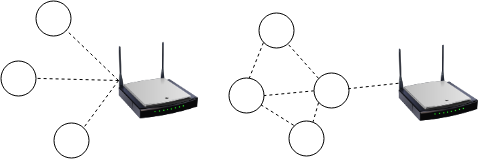
\includegraphics[width=\linewidth]{images/wsn}
	\caption{On the left are IoT devices connecting directly with a dedicated router, and on the right the IoT devices form a WSN in order to reach the router.}
	\label{fig:wsn}
\end{figure}

IoT devices are often restricted by battery life, memory, and computational capabilities. This makes reducing communication overhead and the amount of bookkeeping the main goals for most routing protocols in WSNs. However, most IP routing protocols focus on finding the shortest route between a source and destination, which often results in a small number of paths being heavily used and so some nodes are especially drained due to processing and forwarding of packets. WSNs also experience more mobility than wired networks, which requires more update messages to be flooded throughout in order for packets to be routed correctly. This can result in a network partion once crucial nodes fail (due to loss of battery), rendering a section of still operational nodes useless. An approach to routing and addressing that reduced the networking overhead and attempted to balance traffic across several paths would allow IoT networks to remain operational for longer. 

\begin{figure}[!ht]
	\centering
	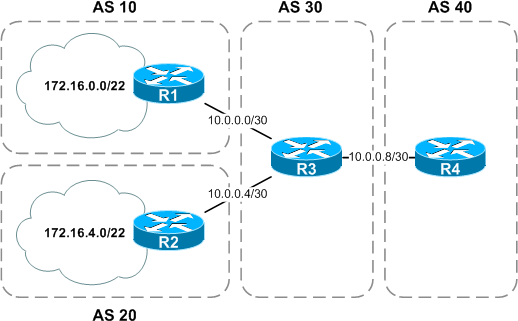
\includegraphics[width=0.8 \linewidth]{images/agg}
	\caption{Example of address aggregation (Image from \cite{agg})}
	\label{fig:agg}
\end{figure}

IPv4 is currently still the most used addressing scheme, and despite the imminent exhaustion of IPv4 addresses \cite{ripe_labs}, IPv6 is being adopted slowly \cite{google_ipv6}. One of the main issues with IP addresses is the fact that they are used to both identify a system and to determine its topological location. \cite{briancarpenter2014} lists several of the downsides to this overloading of IP addresses, and why the protocol was still adopted despite them. 
For the variety of topologies and dynamic nature of WSNs, this overloading causes many issues. Usually when using IP, routers are able to perform address aggregation to reduce how many addresses they have to record for forwarding purposes, like in figure \ref{fig:agg}. But in cellular networks like those used by mobile phones for example, the path to the devices that packets need to take is constantly changing, and so mechanisms such as network address translation (NAT) and complex protocols such as Mobile IP need to be implemented. 

Due to the inability to aggregate addresses, the scalability of the internet is being challenged. An IAB workshop \cite{rfc4984} detailed how the DFZ RIB databases are growing in size exponentially due to the increasing number of devices and an inability to perform address aggregation. One of the main causes of this inability is traffic engineering. In order to improve reliability, many ISPs are using multipath routing with the intention of balancing load. This improves network performance for the operators that use them, but with IP it places greater stress on the default-free zone (DFZ) routing information base (RIB). Multihoming is also being used to improve reliability, but with IP this requires routing entries to store multiple addresses for one host. 

Given the difficulty involved in migrating from IPv4 to IPv6, it is very doubtful that introducing an entirely different protocol for the internet would be successful. A backwards compatible solution would likely be the only solution that would be adopted within a reasonable time frame. Since so many issues with IP are due to the overloading of the IP address, the alternatives that are being considered use an locator-identifier split approach. 

\begin{figure}[!ht]
	\centering
	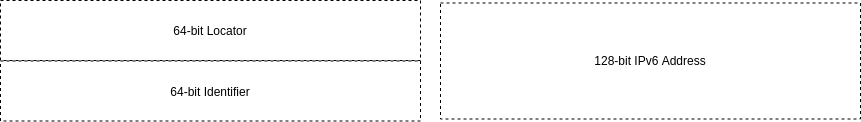
\includegraphics[width=\linewidth]{images/addresses}
	\caption{}
	\label{fig:addresses}
\end{figure}

Both multihoming and mobility are far simpler to implement and maintain if the identity and topological locator of a host are separated, and this is how the Identifier-Locator Network Protocol functions. \cite{5586444} proposes ILNPv6, which implement ILNP with the same address space as IPv6 and the same packet structure as IPv6, but with different semantics for interpreting the addresses. ILNPv6 splits the original 128-bits used for an IPv6 address into two 64-bit fields: the upper bits representing the locator and the lower 64 bits representing the identifier (figure \ref{fig:addresses}). The version field in the IP header is used to differentiate between ILNPv6 and IPv6 packets, and routers that don't support ILNP can interpret the packets as IP without any issue. 

The locator value identifies the subnetwork that a host belongs to, and a host can have multiple locator values, providing multihoming. The ID part of the address is unique to the host, and provides a fixed address which can be used at the transport layer. Because of this, ILNP is well suited to WSNs. Sensors are able to change locators without any changes to their transport layer address, and routing tables can store paths to locators rather than attempting to aggregate addresses in a dynamic topology.

Though ILNPv6 is very backwards-compatible, there are still some difficult challenges involved in its deployment. \cite{ipwithoutip} describes how the tight coupling of the C socket API and IP addresses could cause issues in some legacy applications. ILNPv6 also requires some additions to the Domain Name System (DNS) to properly support multihoming. 

The main goal of this project is to produce a library for a prototype communication
protocol for wireless Internet of Things (IoT) devices based on the identifier-locator approach. By providing a libary for future developers and researchers to use, the adoptation of ILNP could be accelerated. With the ability to emulate networks that use ILNP, routing protocols could be designed that optimise for the likely imminent change in addressing scheme. 

For the example routing protocol, an agricultural sensor network scenario was chosen. 

\vspace{\baselineskip}
\noindent A sucessful implementation would include:

\begin{enumerate}
	\item \textbf{Load Balancing}: The protocol will attempt to evenly disperse load across a network of IoT
devices. This could be measured by demonstrating a reasonably even distribution of packets throughout the network of nodes when simulating sensor traffic. 
	\item \textbf{Soft Handovers}: The protocol will attempt to handle ’soft-handovers’, allowing nodes to
move between subnetworks and handle node failure without a noticeable effect on performance. A successful implementation will recover from failed nodes, with messages still arriving reliably. This could be tested by emulating network traffic, and triggering nodes in certain positions in the network topology to fail.

	\item \textbf{IoT Optimization}: The protocol will account for battery usage on devices to reduce energy drain
	on devices. This will be tested through emulation of an IoT network and the energy cost of packets.
	\item \textbf{ILNP Addressing}: The protocol will be built around the identifer-locator split addressing scheme ILNPv6, and will perform better than IP in the same scenario.
\end{enumerate}

\pagebreak
\section{Context Survey}

Despite the intitial motivation for WSNs being military applications, they are now being used to solve many other problems.

The sensitivity of crops to changes in climate and agricultures crucial role on national economies has naturally resulted in large amounts of research and development. \cite{agrisensor} describe how sensor technology is being used to monitor conditions in greenhouses, fields, and bodies of water. In order to make accessing this data more convenient and to help automate processes, they implemented a wireless network of enviromental sensors. This data would then be collected at a sink node and could be analysed from an application. 

WSNs currently often require specialised applications and manually specified network configurations in order for consumers to collect and analyse the data they produce. In order to make access to the data more standardised and easily available, research is also being done to connect sensor networks to the cloud. \cite{indoor} propose enviromental sensors for urban environments with gateways to to the internet which could integrate into our own homes. By providing cheap montoring and actuating sensors to the general public, they hope to encourage healthier eating habits, as people would be able to grow their own vegetables effectively. 

\cite{wsnlist} list the other applications of WSNs, and the different approaches to integrating WSNs and the internet. They recognise that providing a single gateway results in a single point of failure, and so focus on methods involving multiple or integrated gateways. This requires that sensors adopt the responsiblity of managing their networks topology instead of just forwarding towards a sink node. 

Previous research involving integrating WSNs into the current internet infrastructure is typically structured around IP. For all the reasons mentioned earlier, researches have realised the benefits of building WSNs using other approaches such as the locator-identifier split.

In RFC6115 \cite{rfc6115}, ILNP was listed alongside several other solutions that resolved the issues faced by IP. One of the most well researched solutions listed is the Locator-Identifer Split Protocol (LISP), which has already been deployed in 60 sites over 10 countries \cite{nahla}. Whilst it does not have natural support for network mobility, attempts have been made to provide it that require further extensions to the protocol \cite{moblisp}. 

ILNPv6 on the other hand has been able to demonstrate reliable mobility using a soft handover process \cite{shilnp}. Soft handover is where a host remains connected to it's original network while transitioning to a new one, which avoids loss of data when packets are still being routed to it's original network. 

Soft handovers are crucial for high mobility devices such as smartphones, which are constantly transitioning between networks. Handovers are implemented in Mobile IP for IPv6, and has been improved since IPv4, but the method is still not as performant as it could be. It also further muddies the meaning of IP addresses, due to the use of different addresses (e.g. 'home' and 'care-of' addresses) in order to redirect packets to the mobile node. 

\begin{figure}[!ht]
	\centering
	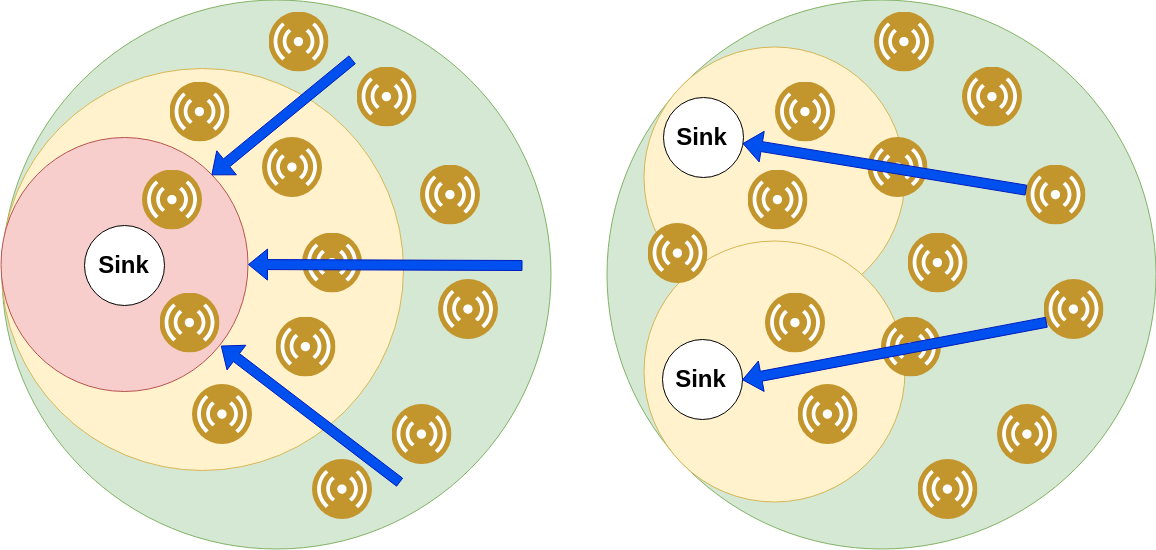
\includegraphics[width=\linewidth]{images/diameter}
	\caption{Comparison between the use of a single sink and multiple sink nodes. Coloured circles represent the amount of traffic (red, yellow, green where red means the high traffic) and the small yellow circles represent transmitting devices.}
	\label{fig:diameter}
\end{figure}

Multihoming is also incredibly useful for WSNs, as it can potentially allow them to scale without being reconfigured. WSN lifetimes are inversely proportional to their diameter when a single sink or gateway is available \cite{multisink}. By providing multiple sinks, the levels of traffic around the sink nodes is decreased, increasing the longevity of the network. With ILNP the end destination identifier could remain the same, and so the underlying routing protocol would only have to include a way of realising a route to the new interface like in the scenario shown in figure \ref{fig:diameter}.

A different addressing scheme is only part of the solution required for successful intergration of WSNs and the internet. Due to the myriad of situations that IoT devices are used, there is no one-size-fits-all solution, and so many versions of IoT routing have been proposed.

\cite{hassan} classifies different routing protocols and provides a survey of protocols for each class. Routing protocols are either proactive, reactive, or hybrid. 

Proactive protocols maintain knowledge of the network topology using regular flooding and beacon messages. This is acceptable for most of the internet infrastructure, but periodic messages can drain precious energy from devices that are power by battery. Since the state of links are always tested, packet delivery is more reliable, and if nodes change position a new path can be built quickly. In the current internet, OSPF is one of the most popular interior gateway protocols, and so naturally researchers tried to adapt it to wireless networks. This produced the Optimized Link State Routing (OLSR) protocol \cite{olsr} and Open Shortest Path First MANET Designated Routers (OSPF-MDR) protocol. However, in low mobility scenarios however, reactive protocols perform far better than either of these options. 

Reactive protocols involve only seeking out routes to destinations when one is required. Examples include AODV \cite{aodv} and DSR \cite{dsr}. These protocols were designed for mobile ad-hoc networks, and so most research involves improving them to be aware of energy availability. For example, \cite{eaodv} produced a solution that considered the mean energy of a path before choosing which route to suggest to the requesting node. This would discourage the use of paths where nodes had low energy reserves. By doing so, less route repairs need to occur, and network partions are postponed. Reactive protocols are also well suited to the wireless medium, as the lack of periodic updates reduces the chance of interference which exists with proactive protocols.

In order to balance reliability and scaling with overhead, a hybrid approach can be applied. For example, \cite{cluster} use a clustering approach in order to manage resources within subsets of nodes. Since not all WSNs are homogenous, this approach can take advantage of some nodes having larger energy reserves than others by electing these nodes as the coordinator of the subnetwork. \cite{vanet} also implement a hybrid routing protocol for vehicle mobile networks which uses beacons to monitor link states between nodes to allow recovery to occur when the routes created by the proactive protocol fail. They also use GPS to help route packets when their target is in a known location. Both these implementations use IP, but grouping nodes by locator and calculating locators on GPS coordinates could be done with ILNP in a more effective way, which is why providing an emulation tool for ILNP ad-hoc networks would be beneficial to research.

\pagebreak
\section{Protocol Design} \label{protodesign}

\subsection{Motivation and Overview}

The protocol used is a reactive zone-based routing protocol (ZBR), and is based on the work by \cite{zbrp} with added support for energy awareness. It was designed with the following assumptions:

\begin{enumerate}
	\item All nodes have equal computation and network ranges.
	\item All nodes that share a locator are also physically located in a simliar area.
	\item Locators cover a similiar physical area, in a lattice structure.
\end{enumerate}

The scenario this protocol was designed for involved agricultural sensor networks. These often consist of many sensor nodes for monitoring the environment and a few actuators for triggering sprinklers or covering delicate crops. Based on the data collected by sensors, they could control the actuators within their locators themselves, whilst reporting their readings to the sink for further analysis. By splitting sensors into geographically relevant zones and assiging locators using tools such as GPS, the arriving data could also be grouped by origin location to help with visualisation and analysis at the sink. 

\begin{figure}[!ht]
	\centering
	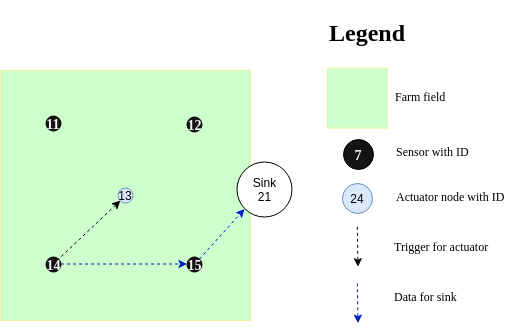
\includegraphics[width=0.8\linewidth]{images/actuate}
	\caption{Communication patterns in agricultural WSN}
	\label{fig:actuate}
\end{figure}

Figure \ref{fig:actuate} provides an example of communication where a sensor wants to trigger some behaviour at an actuator node, and also sends its readings to the sink node. 

In this scenario, the only knowledge that would be available upon initialization of a sensor is its ID and locator, and the ID of the sink node. Sensors would detect any other hosts within their subnetwork, which could be devices such as sprinkler systems, shelters, or cameras. If the sink node was not part of their subnetwork, then they would need to locate it.

In order to scale for large farms, this zone based protocol uses a different routing strategy for routing within and between locators, referred to as the intrazone and interzone routing protocols (IARP, and IERP). The IERP is based on the reactive protocol AODV, and the IARP is based on the link state protocol OLSR with added fields to try and account for energy usage in paths. 

A reactive protocol was chosen for communication between locators in order to limit the amount of network knowledge required for routing. It also has the benefit that link breakages do not need to be broadcast to the entire network, and can instead only be sent to nodes relying on that links existence at the time of breakage.

A proactive protocol was chosen for routing within locators as it would provide node discovery, and would hopefully reduce the number of repeated route discoveries after breakages by being able to find alternative routes within locators. Whilst the keepalives may affect battery life, the static nature of such a network would allow for a large delay between them, making their effect neglible.

\subsection{Intra-Zone Routing Protocol}

Initially, each node broadcasts its presence to its neighbours in order to learn what links were available to it using a \emph{Hello} message, containing its lambda value. 

Neighbouring nodes reply with their current link state database (LSDB) in a \emph{LSDBMessage}. This message contains the neighbouring nodes knowledge of the internal (within the locator) topology, as well as the links to external networks (other locators). Whilst still in the intiliziation phases, neighbours will flood their entire LSBs to their neighbours until no more changes are detected. At this point they can be considered initialized. This ensures that every node in the network has the same database and is aware of all other nodes in the network.

The LSDB messages also provide a metric for choosing paths based on their energy levels. Each node calculates a value $\lambda$ using equation \ref{eq:lambda}, which is visualised in Figure \ref{fig:lambda}. 

\begin{equation} \label{eq:lambda}
	\lambda = 1 -(1 - E)^2
\end{equation}

where $E$ is the \% battery remaining. It is based on the equation for $\lambda$ in \cite{groups}, adjusted so that $E = 0$ occurs when the battery is empty. 
The effect of decreasing $E$ was chosen so that the value of $\lambda$ would be similiar during network initialization, and would gradually become important as the $E$ decreased.

\cite{groups} also included a load balancing factor that would account for the number of neighbours a node had, and this was considered for use in the this implementation, but was not implemented.

\begin{figure}[h]
	\centering
	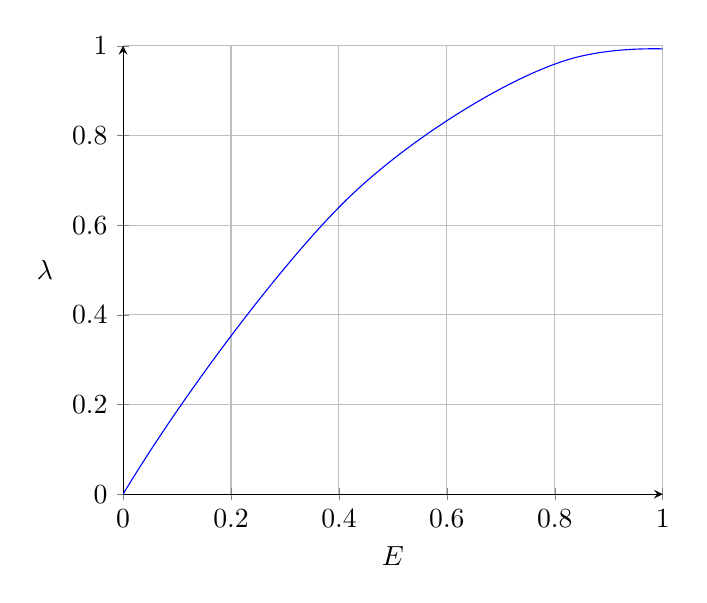
\begin{tikzpicture}
%		\begin{axis}[set layers,view={90}{0},
%			 axis lines=left,
%			 grid=major,
%			 no marks,
%			 xmin=0, xmax=1, xlabel=$E$,
%			 ymin=0, ymax=1, ylabel=$\lambda$, ylabel style={rotate=-90}
%			 ]
%			\addplot+[smooth,blue] {1 - (1 - x)^2}; % actual curve
%			\begin{pgfonlayer}{pre main}
%				\clip plot[variable=\x,samples=25,domain=0:1] (\x,{1 - (1 - \x)^2})
%				|-cycle;
%				\node at (0.5,0.5){\usebox\backbox};
%			\end{pgfonlayer}
%			% filling
%		\end{axis}
		\begin{axis}[set layers,view={90}{0},
			 axis lines=left,
			 grid=major,
			 no marks,
			 xmin=0, xmax=1, xlabel=$E$,
			 ymin=0, ymax=1, ylabel=$\lambda$, ylabel style={rotate=-90}
			 ]
			\addplot+[smooth,blue] {1 - (1 - x)^2}; % actual curve
		\end{axis}
	   \end{tikzpicture}
	   \caption{Plot of Equation \ref{eq:lambda}}
	\label{fig:lambda}
\end{figure}

Nodes that exist on the border of locators will discard LSBs they receive from the locators they are not part of. They will however use these messages to learn what other locators can be reached from their neighbours, eventually providing them with next hops for all locators in the WSN.

Once converged and the entire local topology is available, data packets would be routed using the following logic:

\begin{enumerate}
	\item If the packet destination ID matches the current node, then it will add the payload of the packet to the received queue. 
	\item Otherwise it will attempt to find the next hop for the packet, provided by the forwarding table, and forward it to the node with that ID. 
	\item If no entries are found in the forwarding table:
	\begin{enumerate}
		\item If the packet destination locator matches this nodes locator, then not finding a next hop suggests that the destination ID doesn't exist, and so the packet is discarded. 
		\item Otherwise, the inter-zone routing protocol will be invoked, but only if the packet originates from the current node. 
	\end{enumerate}
\end{enumerate}

This method ensures that packets arriving from external locators will receive best effort routing based on the assumptions that:

\begin{enumerate}
	\item All nodes within a locator have at least one path between each other. 
	\item Data packets are only sent to other locators once a route has been established.
\end{enumerate}

With the link state databases synchronised, nodes then begin periodically sending keepalive messages. Figure \ref{fig:helloflow} shows how these messages are processed. 

\begin{figure}[!ht]
	\centering
	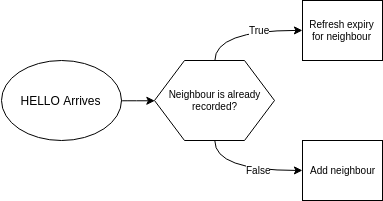
\includegraphics[width=0.6\linewidth]{images/helloflow}
	\caption{Keepalive (hello) flow.}
	\label{fig:helloflow}
\end{figure}

Whenever a link is detected as being lost due to the lack of keepalive messages after a period of time, then this information will be shared within the network. A \emph{ExpiredLink} message will be broadcast, and flooded by nodes within the same locator in order to remove the link from their network, or to inform the other nodes that a neighbouring locator is no longer accessible via a given link.

\begin{figure}[!ht]
	\centering
	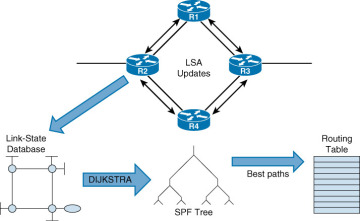
\includegraphics[width=\linewidth]{images/ldb}
	\caption{Intra-zone routing protocol process (image credit \cite{ldb}}
	\label{fig:lsbexchange}
\end{figure}

The internal forwarding table is constructed from the link state database messages as shown in figure \ref{fig:lsbexchange}. The network graph is converted to a forwarding table by constructing a shortest path tree. In the case where two equal length paths exist between this node and a destination, the one with the best value for $\lambda$ will be chosen for the next hop. The forwarding table also caches the locators for nodes outside of the current locator so that route discovery is not repeated unnecessarily.

\subsection{Inter-Zone Routing Protocol}

The inter-zone routing protocol is based on AODV, which is a reactive protocol. AODV typically has three phases (route discovery, maintenance, and repair), but in this implementation route discovery also provides locator discovery.

Locator discovery is necessary since locators are not known for all nodes in the network. Usually the DNS would provide the locators for a given identifier or fully qualified domain name (FQDN), but since that is not a practical option for a wireless sensor network, the locator will have to be found manually. 

To discover routes to a given ID, a route request is made. A node will create a route request and forward a copy towards each of neighbouring locators. The first node that receives the request in each locator will check if the destination ID is in their subnetwork, and if so they will reply. Otherwise, they will forward it to any neighbours that have not already been added to the hop list. The route discovery process is summarised in figure \ref{fig:path}, where a node from the leftmost locator (1) is requesting a route to a node in the the rightmost locator (4).

\begin{figure}[!ht]
	\centering
	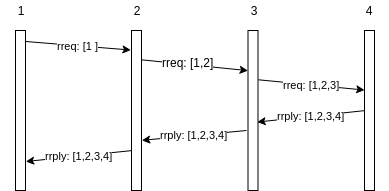
\includegraphics[width=\linewidth]{images/path}
	\caption{Route discovery made by a node in locator one for a node that is found in locator 4.}
	\label{fig:path}
\end{figure}

Figure \ref{fig:rreqflow} shows how RREQs are processed at each node. The destination node replies to all route requests for it, as this can provide multiple paths to the requesting node. Intermediate nodes however only forward requests based on whether or not they've seen them already. This can be established based on the request ID in the RREQ message, which coupled with the source ID in the ILNP packet header can identify duplicate requests. Usually in AODV, route requests are flooded to all nodes. In this implementation, route requests are unicasted to border nodes instead in order to reach other locators. 

When using ILNP instead of IP with AODV, packets can be routed based on the identifier alone, and this can result in multiple paths to the same node. This provides robust communication if the end destination is multihomed (i.e. has interfaces to multiple locators), with less complexity than in IP. 

\begin{figure}[!ht]
	\centering
	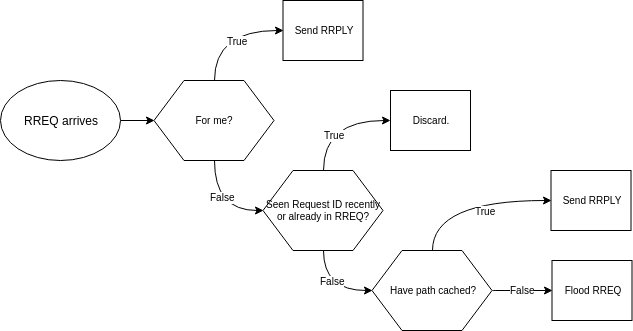
\includegraphics[width=\linewidth]{images/rreqflow}
	\caption{Route Request (RREQ) Flow}
	\label{fig:rreqflow}
\end{figure}

Once the RREQ reaches its destination, or any intermidiate node that already has a path cached to the that destination, a Route Reply (RRPLY) is generated by copying the full path from the RREQ or route cache and sending it back along the same path it arrived to the requesting node. Figure \ref{fig:rrplyflow} shows the processing that occurs at each node.


\begin{figure}[h]
	\centering
	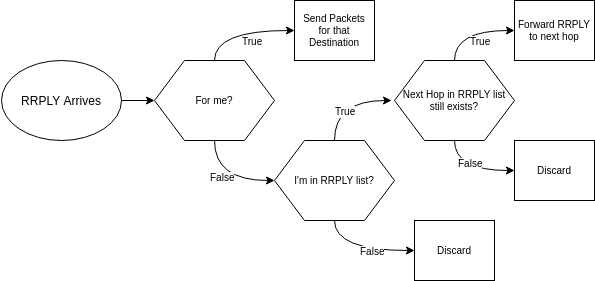
\includegraphics[width=\linewidth]{images/rrplyflow}
	\caption{Route Reply (RRPLY) Flow}
	\label{fig:rrplyflow}
\end{figure}

By forwarding RRPLYs along the reverse of the path that they contain, we ensure that the route hasn't broken between creation and reception of the route request. Intermediate nodes can filter erraneous route replies by only considering those where they know the next hop neighbour is still available.

This only works if we assume that all links are bidrectional which is not always the case especially in heterogenous WSNs, due to differences in transceiver ranges. 
\cite{unidirec} shows that accounting for unidirectional links in a protocol does not provide much benefit compared to the increased overhead. Also in our scenario, the nodes are likely to be homogenous and evenly spaced, so transceiver power can be assumed to be equal throughout, with no interference hot spots. 

\begin{figure}[!ht]
	\centering
	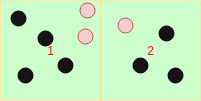
\includegraphics[width=0.5\linewidth]{images/nb}
	\caption{Border Nodes (Red)}
	\label{fig:border}
\end{figure}

If multiple border nodes (nodes that have links to another locator) provide links to the same neighbour zone, then they will will alterate between them using a weighted round robin method based on the path costs to avoid all traffic travelling through the same border node. For example, in figure \ref{fig:border} there are two links from locator 2 to locator 1, and so either can be used.

When packets arrive to be forwarded to another locator, the interzone forwarding table will be used to find the next hop locator. Then the intrazone forwarding table will be used to provide the next hop ID in order to reach a border node that can get the packet closer to the destination locator;

Figure \ref{fig:external} shows the full locator discovery occuring, which returns the locator of the destination node with the requested ID, and the hop by hop list of locators that have to be crossed to reach it.
Once this locator discovery has been carried out, border nodes will be aware of how to reach each locator, and so will be able to forward packets to that destination.

\begin{figure}[!ht]
	\centering
	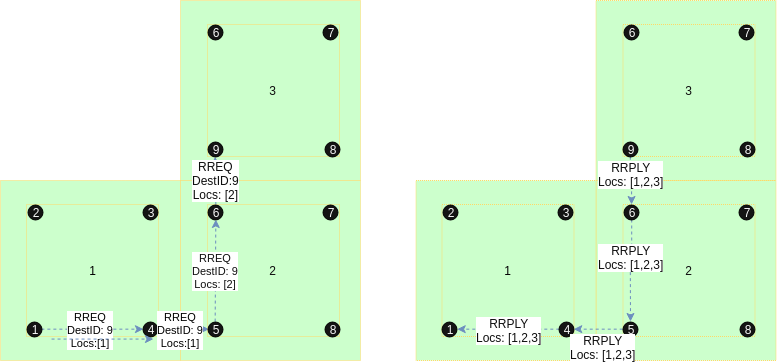
\includegraphics[width=\linewidth]{images/external}
	\caption{Locator Discovery where node 1 needs a route to node 9. The black numbered circles each represent a node with an ID, and the green squares are locators.}
	\label{fig:external}
\end{figure}

If the keepalive process fails for a neighbour and two locators in the route are no longer linked, then a node will forward a RERR to all previous nodes in any paths it takes part in, shown in figure \ref{fig:rerrflow}.

\begin{figure}[h]
	\centering
	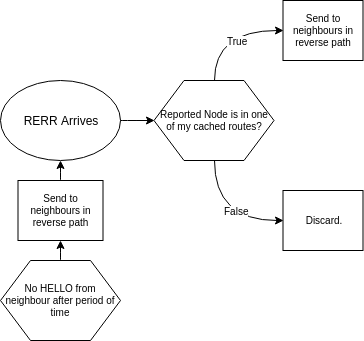
\includegraphics[width=\linewidth]{images/rerrflow}
	\caption{Route Error (RERR) Flow}
	\label{fig:rerrflow}
\end{figure}

Any packets that were sent between the failure of the link and the receiving of a route error will most likely be dropped, and future packets will be delayed as route discovery will have to take place again unless this node is aware of a disjoint path to the destination.

\FloatBarrier
\pagebreak
\section{ILNP Testbed Implementation}

Due to the recency of ILNPv6, there does not currently exist software for emulating wireless ILNP networks as there is for IP, therefore a custom testbed had to be implemented.  

The testing environment was implemented using Python 3.7. The project has three main components: The wireless network emulation, routing and network management, and sensor emulation. Figure \ref{fig:layers} shows how each of these components correspond to a section in the network model.

\begin{figure}[!ht]
	\centering
	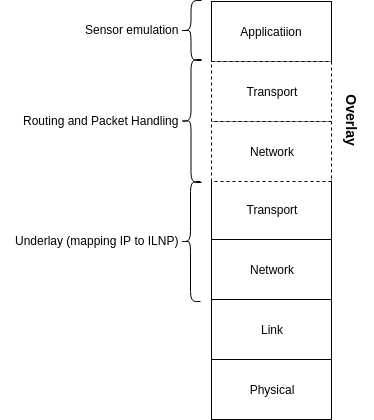
\includegraphics[width=0.7\linewidth]{images/layers}
	\caption{Structure of project with regards to the network model.}
	\label{fig:layers}
\end{figure}

\subsection{Wireless Network Emulation}

Emulating wireless communication was achieved by building an overlay network using UDP with multicast. A single UDP socket provided a communication endpoint.

A multicast group exists for each node ID, and so neighbours of a node would join the multicast groups of their neighbours in order to receive broadcasted packets. Figure \ref{fig:mcast} shows the ranges of each sensors radio signal as dashed lines, where each node within the range joins the multicast group.

\begin{figure}[!ht]
	\centering
	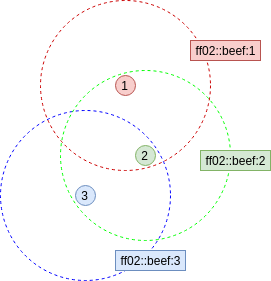
\includegraphics[width=0.5\linewidth]{images/mcast}
	\caption{Wireless broadcast emulation using multicast}
	\label{fig:mcast}
\end{figure}

IPv4 uses the Address Resolution Protocol (ARP) and IPv6 uses Neighbour Discovery (ND) in order to produce a mapping between IP addresses and the link layer addresses of other machines in a local network. In our overlay network, the IP addresses of the underlying network could be treated as MAC addresses. This would allow us to emulate neighbour discovery in ILNPv6, and provide unicast communication once a mapping between these virtual link layer addresses and ILNP IDs were obtained via broadcasted messages. 

The network interface abstraction provided the following methods:
\begin{enumerate}
	\item \textbf{send}: For unicast communication.
	\item \textbf{broadcast}: For establishing neighbours or flooding packets.
	\item \textbf{receive}: For receiving packets, broadcast or unicast.
\end{enumerate}

A daemon thread continuously polls the network interface for incoming data. It then parses the contents of the packet and records the source IDs and source IP addresses of any neighbourhood discovery packets for later communication. Each message type has its own class with its own implementation of \emph{\_\_bytes\_\_} and \emph{from\_bytes()} which would allow them to be serialized from the arriving bytes. To reduce copying and speed up array splicing, memoryviews were used often.

All polling functions included a timeout in order for each thread to check if it has been asked to terminate, if for example the power levels had reached a critical level. If so, a monitor object shared between all threads would be used to trigger a clean shutdown.

\subsection{Routing and Network Management}

The router polls the queue of parsed packets and decides the next course of action. It attempts to route data packets using the current forwarding tables, and hands off control packets to the control plane. 

The control plane handles any control packets or any packets that can't be forwarded using the current forwarding table, and is responsible for populating the forwarding table. It also has a daemon thread which performs maintenance tasks such as aging and retrying route requests, sending keepalives, and monitoring links with neighbours.

The interzone module provides the handler methods for the inter-zone routing protocol. It buffers packets waiting for a route reply for a given destination and handles the forwarding and processing of any inter-zone protocol messages.

The ILNPPacket class when serialized is identical to that from the ILNPv6 RFC. In order to differentiate between control packets and data packets, the payload of the ILNPPacket would be wrapped in a ControlMessage class. Typically control packets and data packets would arrive on seperate ports, but this was not the solution adopted for this implementation.

\subsection{Sensor Emulation}

The sensor initialises the ILNPSocket, and depending on whether or not it is configured to operate as the sink (where all the data from every node is collected) begins either polling for packets or sending 'readings' at intervals.

To mock realistic application data, a random fluctuation is applied to a series of values that would be relevant in our scenario: temperature, humidity, pressure, and luminosity \cite{agrisensor}.

The monitor object shared throughout the project tracks any packets that are sent, and the sink also tracks any readings that it receives. These are then written to a file once the socket is closed for analysis.

\pagebreak
\section{Experiment}

The aims of the experiment were to show that protocol succeeded in meeting the goals described in the introduction. This was be achieved by simulating a wireless sensor network for monitoring fields in a farm. Figure \ref{fig:layout} shows the layout of the scenario being tested. 

\begin{figure}[!ht]
	\centering
	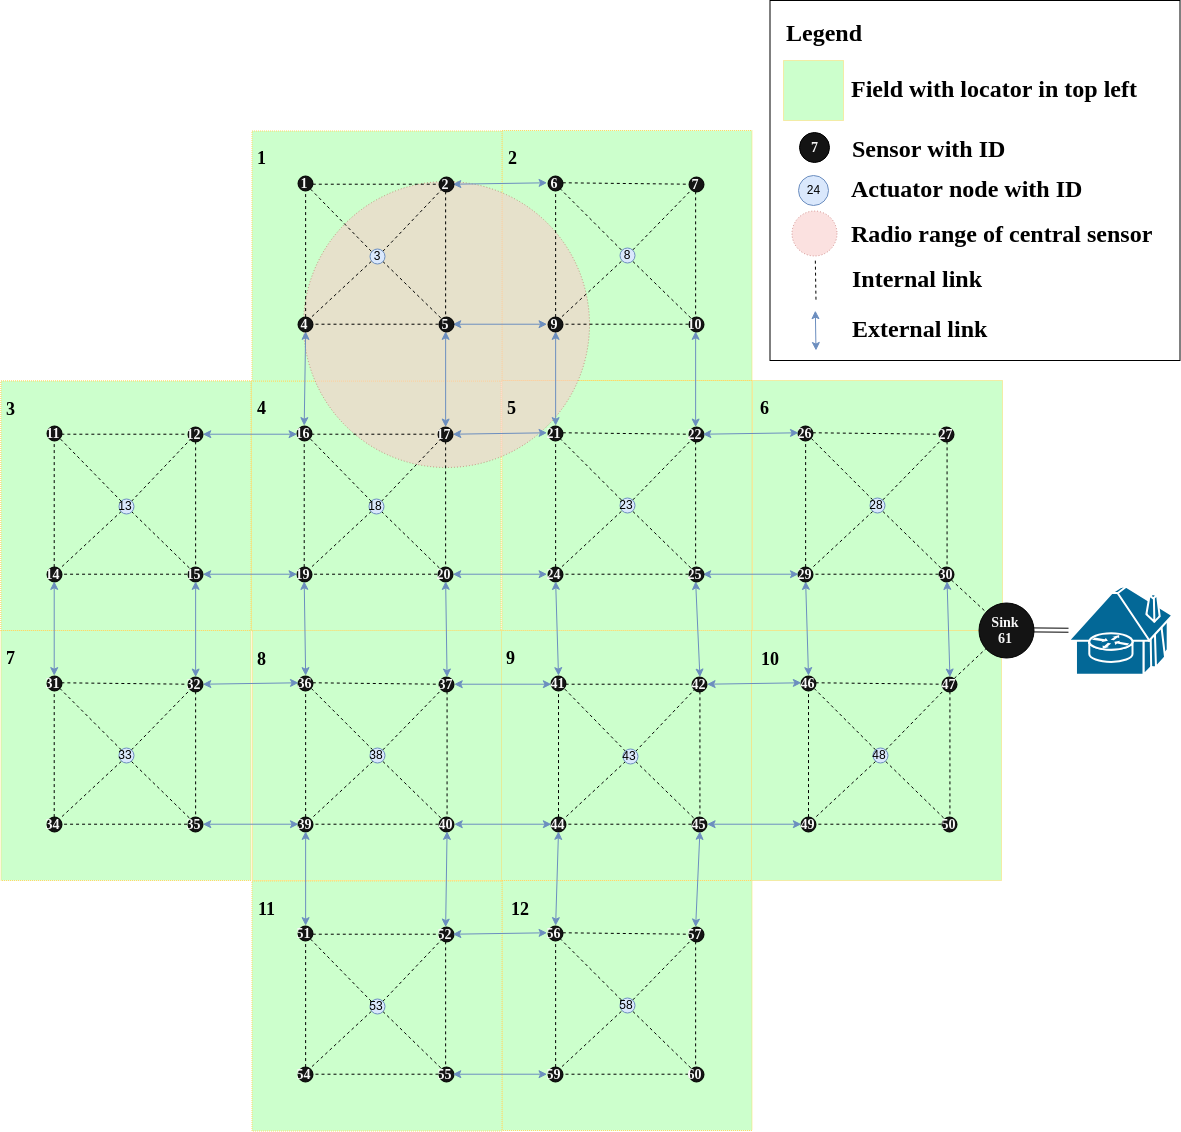
\includegraphics[width=\linewidth]{images/layout}
	\caption{WSN layout with example routes.}
	\label{fig:layout}
\end{figure}

For the emulation, we assumed that: 
\begin{enumerate}
    \item Each sensor had equal radio ranges.
    \item Sensors always listened for packets with same antennae (i.e. no lower power antennaes would be used until a signal was detected\cite{offon})
    \item Sending a packet has a fixed energy cost, regardless of size of payload.
    \item Collisions and interference would not occur.
\end{enumerate}

Two experiments would be run in order to compare performance when using ILNP and IP. Figure \ref{fig:spectrum} shows that ILNP can emulate IP by either:
\begin{enumerate}
	\item providing a locator for every node, essentially treating every node as a subnetwork.
	\item using the same locator for all nodes, which would require knowledge of the entire subnetwork in order to route correctly.
\end{enumerate}

Both extremes of the spectrum will provide identical flat addressing schemes like IP, but would behave differently under the implemented protocol. Using a locator per node basically reduce to AODV, and using a single locator would reduce to OLSR. Figure \ref{fig:spectrum} shows the effect of changing the ratio of locators to nodes.

\begin{figure}[!ht]
	\centering
	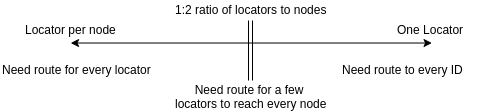
\includegraphics[width=\linewidth]{images/spectrum}
	\caption{Behaviour as the ratio of locators to nodes is changed.}
	\label{fig:spectrum}
\end{figure}

\subsection{Setup}

The experiment was run on the lab machines, remaining within the schools network. 

To construct and automate the testing environment, a series of bash scripts were written. The first of which would perform a quick liveness check by pinging a list of lab machine IP addresses and constructing a list of the IP addresses that responded.

Since multicast was being used to emulate wireless broadcast, my user ID was used as the second-last octet to avoid collision with other experiments possibly running on the network. This is sourced by the implementation and does not need to be specified in the configuration.

The configuration files that were used to initialize each sensor node were generated by performing string replacement on a template configuration. "LOC\_1\_ID\_2\_MCAST\_1\_2" for example would produce a configuration file for a node with ID 2, locator 1, that was part of the multicast groups "ff02::dead:1" and "ff02::dead:2". Being able to describe network topologies using single strings allowed multiple tests to be configured easily, and possible future work could involve generating these configurations using a visual representation of the network.

With the list of available computers and the configuration files generated, another script was written that would \emph{ssh} into the lab machines one by one and start the sensor emulation program with each configuration. Logs from each instance of the program were redirected to a file based on the node ID for monitoring the network.

\subsection{Method}

In order to monitor the type and number of packets sent and forwarded by each node, an additional \emph{monitor} module was added to the testbed implementation. For each packet sent, the monitor recorded a the ID of the sensor, timestamp, the type of packet (control or data), and whether or not the packet originated from this node or was being forwarded. Using this information, the flow of packets over time could be visualised, and the ratio of control packets to data packets (i.e. overhead) could be measured. 

The sink node would also record each data packet it received in order to measure loss. Loss would be calculated from the difference between the number of data packets sent by each sensor and the number received by the sink. 

Each test was run multiple times in order to ensure that the results were consistent.

\subsection{Results}

\textbf{ILNP}

\noindent Figures \ref{fig:datasnapone} to \ref{fig:ctrlsnapthree} show the concentration of data and control packets throughout the network over the period of three equally sized snapshots.

In figure \ref{fig:datasnapone}, node 19 is able to immediately send packets to the sink and so it shows the highest data packet traffic. From the log files it is also evident that it is forwarding packets from the adjacent nodes in its locator. Figure \ref{fig:ctrlsnapone} shows an increase in control packets from nodes in locators further from the sink, as they need to perform locator discovery to find the sink node. In the next snapshot, we can see the effect of route replies as large burst of data packets and route replies are being forwarded by nodes 5 and 9. In the final snapshot, we can see that node 19 has failed. The rest of the network does not appear to recover as node 15 (the only remaining link to the sink) is not forwarding any more traffic than before.

\medskip
\noindent\textbf{IP}

\noindent Figures \ref{fig:ipdatasnapone} to \ref{fig:ipctrlsnapthree} show very different traffic patterns to the ILNP experiment. The control traffic in each snapshot is fairly consistent due to the keepalives, though in the first snapshot the distribution of LSDB messages is not even. Data packets are being sent by each node but mostly for three individual nodes. These abnormal peaks in traffic are likely due to implementation error.

\medskip
\noindent\textbf{Discussion}

\noindent The results do not give much insight into differences between ILNP and IP. They also do not seem to suggest any load balancing or recovery is occuring successfully. However, from the logs it was observed that the sizes of the forwarding tables and network graphs stored by each node are very different. In ILNP, only one locator worth of adresses and a path to the sink is stored, whilst in the IP experiment, both the network graph and forwarding table are large. If the WSN was to be scaled up further, this issue would be exacerbated. The limited memory of IoT devices would place a limit on the size of the network, whilst in this implementation the forwarding table would only be affected by additional nodes within the locator. 

A different approach to the experiment had been considered before using only AODV, and the source code for this will be included in the submission. Whilst that implementation did perform better overall when routing packets in the same network topology than the implementation chosen, it did not make use of the locators in ILNP. The implementation used in this submission was used instead despite being less functional due to the fact that it provided a way to compare IP and ILNP (by changing the ratio of locators to nodes). Given more time to test and debug, the protocol could potential perform very well, but the more interesting design was realised too close to the submission date which left little time for fixes. 

A criticism that can be made of the chosen protocol is that its complexity made development and debugging very difficult. In order to test that it worked correctly, many scenarios had to be recreated. Since arrival times of messages would vary, finding the series of events that led to a problematic state was very time consuming. Verifying the protocol by applying exhaustive model checking would have definitely helped.

It could be argued that this experiment is more a comparison of protocols rather than of the two addressing schemes. WSN protocols have already been proposed that try to organise nodes into clusters and behave very similiarly to this protocol once these clusters are established. With IP however, these protocols require their own addressing schemes which are an abstraction of the underlying IP addresses. ILNP naturally supports grouping in protocols which means this abstraction would not be necessary. By reducing the complexity, protocols become easier to verify, test, and maintain. 

\begin{figure}[!ht]
    \centering
    \begin{minipage}{0.45\textwidth}
        \centering
        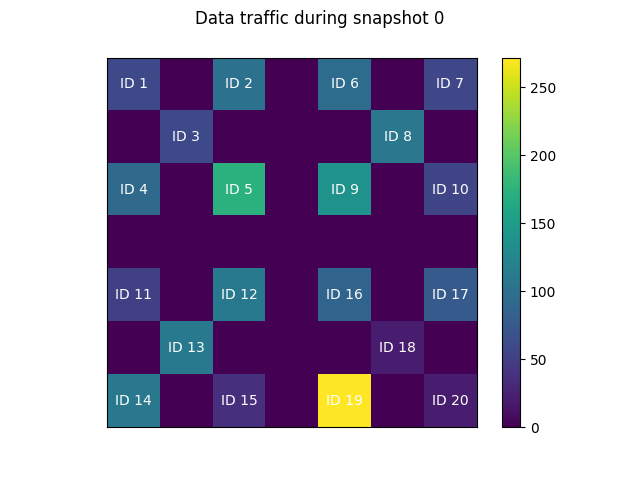
\includegraphics[width=\textwidth]{images/ilnp/snapshot0-Data.png} % first figure itself
        \caption{Data packets sent by each node during network initialisation when using ILNP.}
        \label{fig:datasnapone}
    \end{minipage}\hfill
    \begin{minipage}{0.45\textwidth}
        \centering
        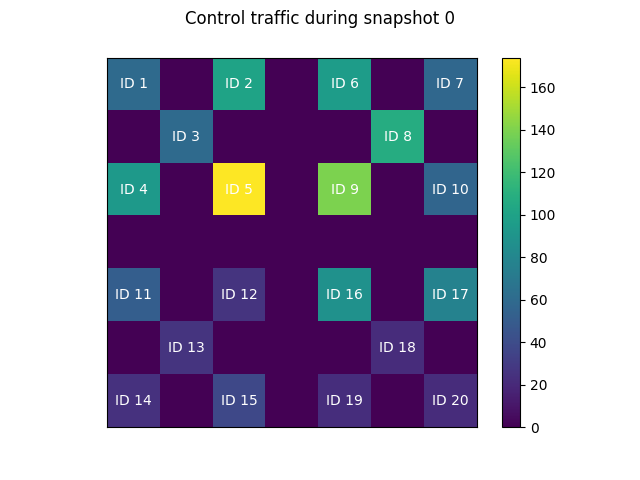
\includegraphics[width=\textwidth]{images/ilnp/snapshot0-Control.png} % second figure itself
        \caption{Control packets sent by each node during network initialisation when using ILNP}
        \label{fig:ctrlsnapone}
    \end{minipage}
\end{figure}

\begin{figure}[!ht]
    \centering
    \begin{minipage}{0.45\textwidth}
        \centering
        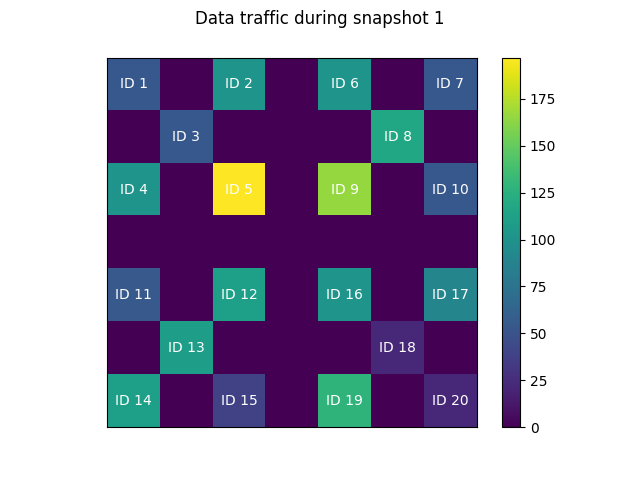
\includegraphics[width=\textwidth]{images/ilnp/snapshot1-Data.png} % first figure itself
        \caption{Data packets sent by each node once initial routes have been established when using ILNP}
        \label{fig:datasnaptwo}
    \end{minipage}\hfill
    \begin{minipage}{0.45\textwidth}
        \centering
       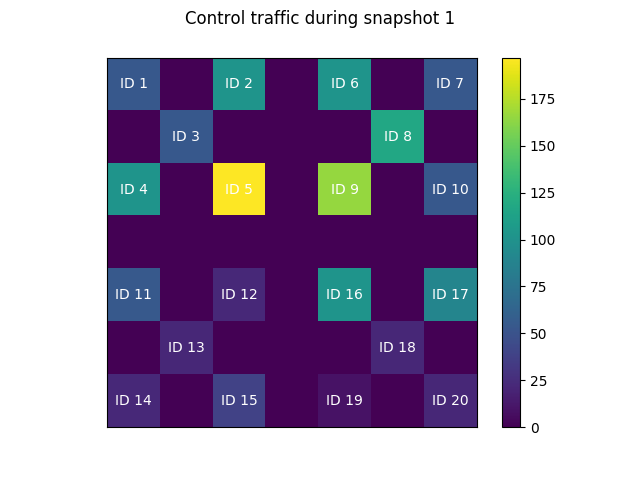
\includegraphics[width=\textwidth]{images/ilnp/snapshot1-Control.png} % second figure itself
        \caption{Control packets sent by each node once intial routes have been established when using ILNP}
        \label{fig:ctrlsnaptwo}
    \end{minipage}
\end{figure}

\begin{figure}[!ht]
    \centering
    \begin{minipage}{0.45\textwidth}
        \centering
        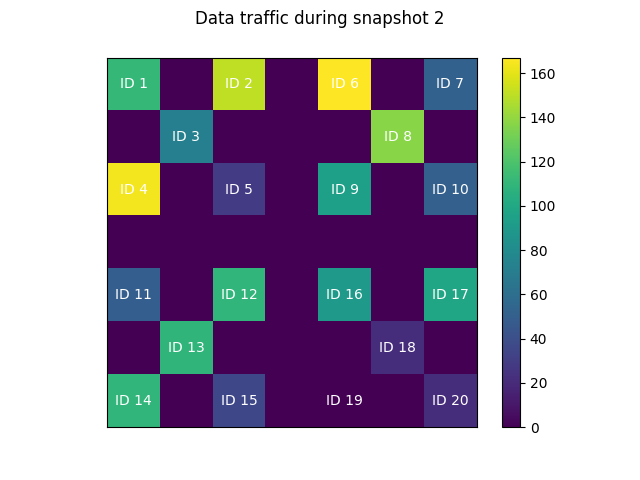
\includegraphics[width=\textwidth]{images/ilnp/snapshot2-Data.png} % first figure itself
        \caption{Data packets sent by each node once failures have started to occur when using ILNP}
        \label{fig:datasnapthree}
    \end{minipage}\hfill
    \begin{minipage}{0.45\textwidth}
        \centering
        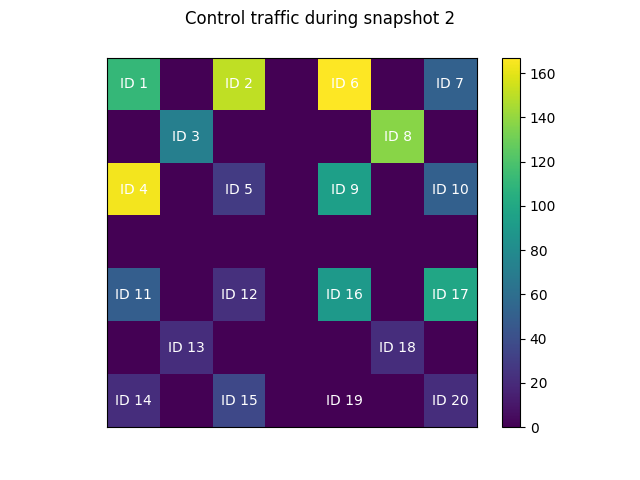
\includegraphics[width=\textwidth]{images/ilnp/snapshot2-Control.png} % second figure itself
        \caption{Control packets sent by each node once failures have started to occur when using ILNP}
        \label{fig:ctrlsnapthree}
    \end{minipage}
\end{figure}


\begin{figure}[!ht]
    \centering
    \begin{minipage}{0.45\textwidth}
        \centering
        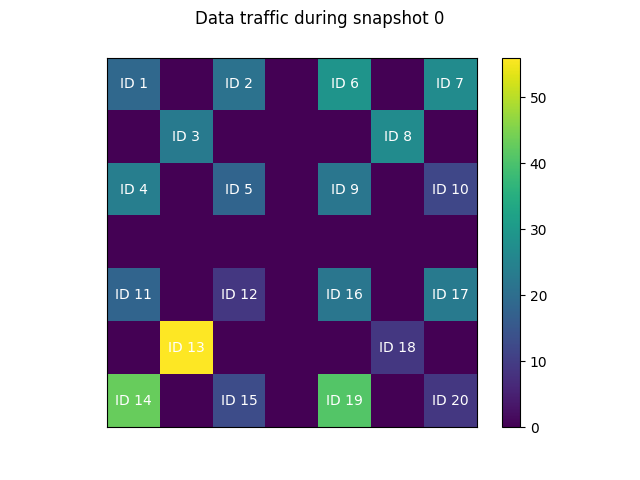
\includegraphics[width=\textwidth]{images/ip/snapshot0-Data.png} % first figure itself
        \caption{Data packets sent by each node during network initialisation when using IP}
        \label{fig:ipdatasnapone}
    \end{minipage}\hfill
    \begin{minipage}{0.45\textwidth}
        \centering
        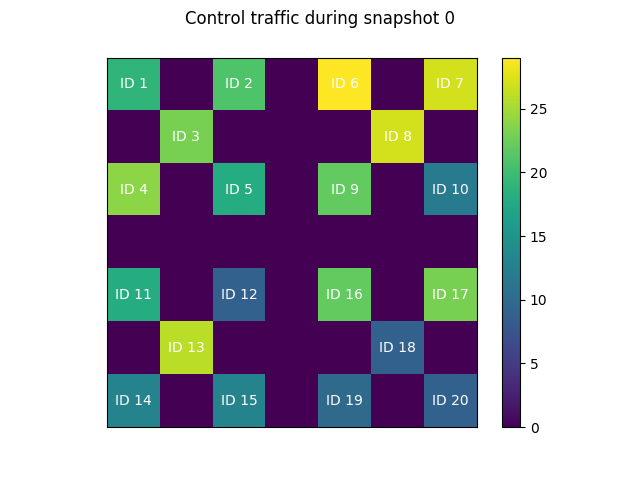
\includegraphics[width=\textwidth]{images/ip/snapshot0-Control.png} % second figure itself
        \caption{Control packets sent by each node during network initialisation when using IP}
        \label{fig:ipctrlsnapone}
    \end{minipage}
\end{figure}

\begin{figure}[!ht]
    \centering
    \begin{minipage}{0.45\textwidth}
        \centering
        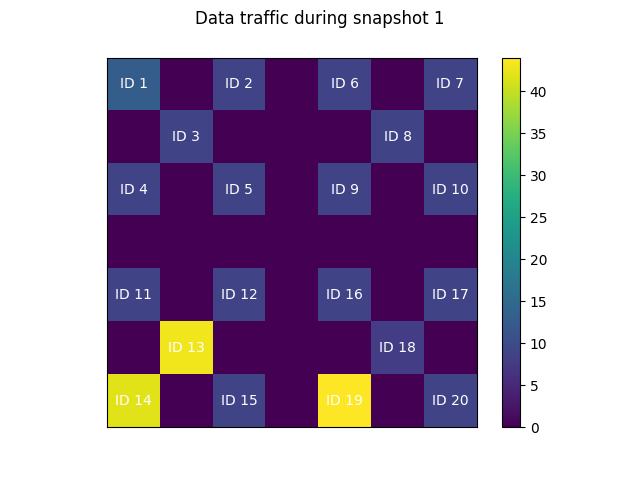
\includegraphics[width=\textwidth]{images/ip/snapshot1-Data.png} % first figure itself
        \caption{Data packets sent by each node once initial routes have been established when using IP}
        \label{fig:ipdatasnaptwo}
    \end{minipage}\hfill
    \begin{minipage}{0.45\textwidth}
        \centering
       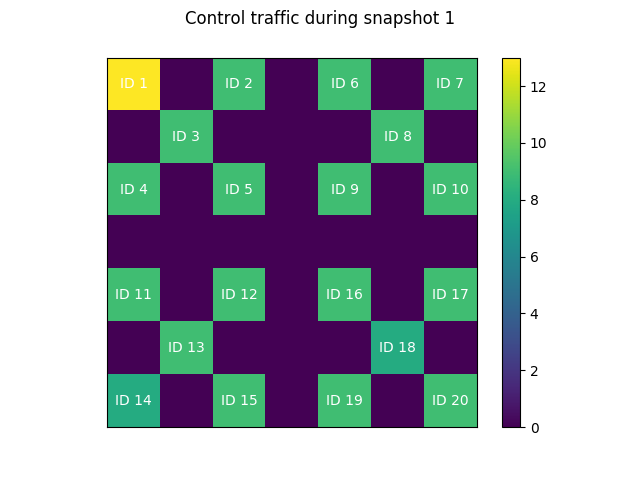
\includegraphics[width=\textwidth]{images/ip/snapshot1-Control.png} % second figure itself
        \caption{Control packets sent by each node once intial routes have been established when using IP}
        \label{fig:ipctrlsnaptwo}
    \end{minipage}
\end{figure}

\begin{figure}[!ht]
    \centering
    \begin{minipage}{0.45\textwidth}
        \centering
        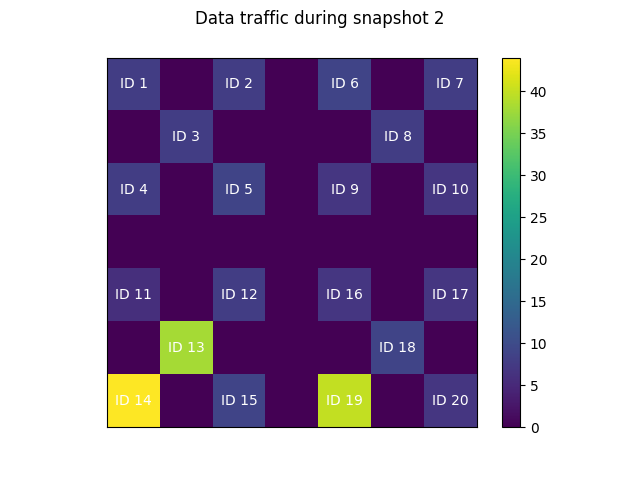
\includegraphics[width=\textwidth]{images/ip/snapshot2-Data.png} % first figure itself
        \caption{Data packets sent by each node once failures have started to occur when using IP}
        \label{fig:ipdatasnapthree}
    \end{minipage}\hfill
    \begin{minipage}{0.45\textwidth}
        \centering
        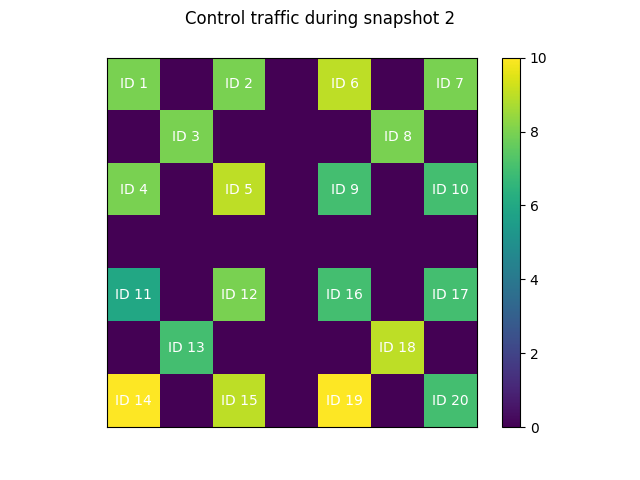
\includegraphics[width=\textwidth]{images/ip/snapshot2-Control.png} % second figure itself
        \caption{Control packets sent by each node once failures have started to occur when using IP}
        \label{fig:ipctrlsnapthree}
    \end{minipage}
\end{figure}

\FloatBarrier
\pagebreak
\section{Conclusion}

Overall, the project was able to meet two of the original four goals. ILNP addressing was adopted successfully, and a protocol optimized for IoT devices was implemented. Due to issues with the end product, the experiments were not particularly useful for comparing ILNP and IP, but did allow for some discussion. ILNP required far less knowledge of the global networks state compared to IP, which could potentially allow WSNs using it to scale further than when using IP. 

Future work that could improve the robustness of the protocol would be to handle the situations where a network partition occurs within a locator. One possible solution would be to allow locators to form dynamically. The implementation used originally featured a mechanism for 'joining' a locator instead of having them statically assigned as in the experiment. By identifying the central node within a locator and setting a maximum radius for each locator, partions within locators could be resolved by both sides of the split attempting to merge with the surrounding locators. This was scrapped from the project due to a shortage of time, but attempts can be found in the version control history.

Security was not considered at all when desigining this protocol, which definitely makes it unsuitable for many situations. It relies heavily on all control messages being legitimate and on the honesty of nodes regarding the ability to forward traffic. For example, if a node with plentiful energy wished to process less network traffic, it could advertise itself as having low energy reserves and be the least likely candidate for forwarding.

The project sufferred due to taking too long to settle on a design, but the process of considering and attempting different variations on ad-hoc routing protocols was very educational. Whilst disappointed that I was not able to get a fully working prototype, the opportunity to work on and resesearch the potential future of the internet proved very interesting.

\pagebreak
\section{Appendix}

\textbf{Running the experiment}
\begin{enumerate}
	\item Update file paths in 
	\begin{enumerate}
		\item \emph{cleanup.sh}
		\item \emph{run\_configs\_on\_machines.sh}
		\item \emph{run\_with\_config.sh}
	\end{enumerate}
	\item Run \emph{get\_up\_machines.sh} to ping all lab machines.
	\item Run \emph{generate\_config\_from\_list.sh configs/\_list.txt name} to generate python configuration file (.ini)
	\item Run \emph{run\_configs\_on\_machines.sh configs/\_list.txt name} to start application on list of machines.

\end{enumerate}

\noindent\textbf{Configuration for ILNP Test}

\begin{lstlisting}
LOC_1_ID_1_MCAST_2_3_4
LOC_1_ID_2_MCAST_1_3_5_6
LOC_1_ID_3_MCAST_1_2_4_5
LOC_1_ID_4_MCAST_1_3_5_11
LOC_1_ID_5_MCAST_2_3_4_9_12
LOC_2_ID_6_MCAST_2_7_8_9
LOC_2_ID_7_MCAST_6_8_10
LOC_2_ID_8_MCAST_6_7_9_10
LOC_2_ID_9_MCAST_5_6_8_10_16
LOC_2_ID_10_MCAST_7_8_9_17
LOC_3_ID_11_MCAST_4_12_13_14
LOC_3_ID_12_MCAST_5_11_13_15_16
LOC_3_ID_13_MCAST_11_12_14_15
LOC_3_ID_14_MCAST_11_13_15
LOC_3_ID_15_MCAST_12_13_14_19_21
LOC_4_ID_16_MCAST_9_12_17_18_19
LOC_4_ID_17_MCAST_10_16_18_20
LOC_4_ID_18_MCAST_16_17_19_20
LOC_4_ID_19_MCAST_15_16_18_20_21
LOC_4_ID_20_MCAST_17_18_29
LOC_4_ID_21_MCAST_15_19
\end{lstlisting}

\noindent\textbf{Configuration for IP Test}
\begin{lstlisting}
LOC_1_ID_1_MCAST_2_3_4
LOC_1_ID_2_MCAST_1_3_5_6
LOC_1_ID_3_MCAST_1_2_4_5
LOC_1_ID_4_MCAST_1_3_5_11
LOC_1_ID_5_MCAST_2_3_4_9_12
LOC_1_ID_6_MCAST_2_7_8_9
LOC_1_ID_7_MCAST_6_8_10
LOC_1_ID_8_MCAST_6_7_9_10
LOC_1_ID_9_MCAST_5_6_8_10_16
LOC_1_ID_10_MCAST_7_8_9_17
LOC_1_ID_11_MCAST_4_12_13_14
LOC_1_ID_12_MCAST_5_11_13_15_16
LOC_1_ID_13_MCAST_11_12_14_15
LOC_1_ID_14_MCAST_11_13_15
LOC_1_ID_15_MCAST_12_13_14_19_21
LOC_1_ID_16_MCAST_9_12_17_18_19
LOC_1_ID_17_MCAST_10_16_18_20
LOC_1_ID_18_MCAST_16_17_19_20
LOC_1_ID_19_MCAST_15_16_18_20_21
LOC_1_ID_20_MCAST_17_18_29
LOC_1_ID_21_MCAST_15_19
\end{lstlisting}

\bibliographystyle{unsrt}
\bibliography{mybib}

\end{document}
